\documentclass[a4paper, 11pt]{article}
\usepackage[polish]{babel}
\usepackage[T1]{fontenc}
\usepackage{hyperref}
\usepackage{array}
\usepackage{amssymb}
\usepackage{amsmath}
\usepackage{changepage}
\usepackage{multicol}
\usepackage[margin=1in]{geometry}
\hypersetup{
    colorlinks,
    citecolor=black,
    filecolor=black,
    linkcolor=black,
    urlcolor=black
}
\usepackage{graphicx}

\usepackage{tikz}
\usetikzlibrary{fit,arrows,matrix,positioning, calc, shapes.gates.logic.IEC, shapes.gates.logic.US}
\usetikzlibrary {arrows.meta}
\tikzstyle{branch}=[fill,shape=circle,minimum size=3pt,inner sep=0pt]


\title{%
        \vspace{-1cm}
       \large Sprawozdanie Laboratorium Fizyka dla informatyków \\
       \huge Wyznaczanie ogniskowych soczewek
ze wzoru soczewkowego oraz metodą Bessela.}

\author{Stanisław Fiedler 160250}
\date{LAB 5, 7 stycznia 2025}

\begin{document}
\begin{table}
	\begin{adjustwidth}{-0.25\textwidth}{-0.25\textwidth}
		\begin{center}
			\begin{tabular}{|l|l|l|l|l|}
				\hline
				Nr Ćwiczenia 302                                             & Data wykonania 07.01.2025                 & Wydział WIiT & Semestr 3 & Grupa LAB L1 \\
				\hline
				\multicolumn{2}{|l|}{ Prowadzący: mgr inż. Taras Zhezhera  } & \multicolumn{2}{|l|}{ Stanisław Fiedler } & Ocena:                                  \\
				\hline
			\end{tabular}
		\end{center}
	\end{adjustwidth}
\end{table}

\maketitle
\tableofcontents

\section{Wstęp teoretyczny}\label{sec:wstep} % (fold)

Soczewką jest ciało przeźroczyste o dwóch powierzchniach sferycznych.
Wiązka promienie biegnąca równolegle do soczewki po przejściu przez nią skupi się w punkcie zwanym ogniskiem.
Dobierając krzywizny buduje się soczewki skupiające i rozpraszające.
Położenie ogniska zależy od współczynnika załamania materiału soczewki oraz promieni krzywizn.
\[
	\frac{1}{f} = (n-1) \left( \frac{1}{R_1} - \frac{1}{R_2} \right)
\]
Soczewki odwzorowują obraz a jego położenie jest opisane równaniem soczewkowym:
\[
	\frac{1}{f} = \frac{1}{p} + \frac{1}{o}
\]
Ogniskową układu soczewek opisuje wzór:
\[
	\frac{1}{f} = \frac{1}{f_1} + \frac{1}{f_2} - \frac{d}{f_1f_2}
\]
Uwzględniając symetrię wzoru soczewkowego i przekształcając go otrzymujemy wzór metody Bessela:
\[
	e = l - o' - p
\]
\[
	f = \frac{l^2 - e^2}{4 \cdot l}
\]

% section wstep (end)

\section{Wyniki pomiarów}\label{sec:wyniki_pomiarow} % (fold)
\begin{center}
	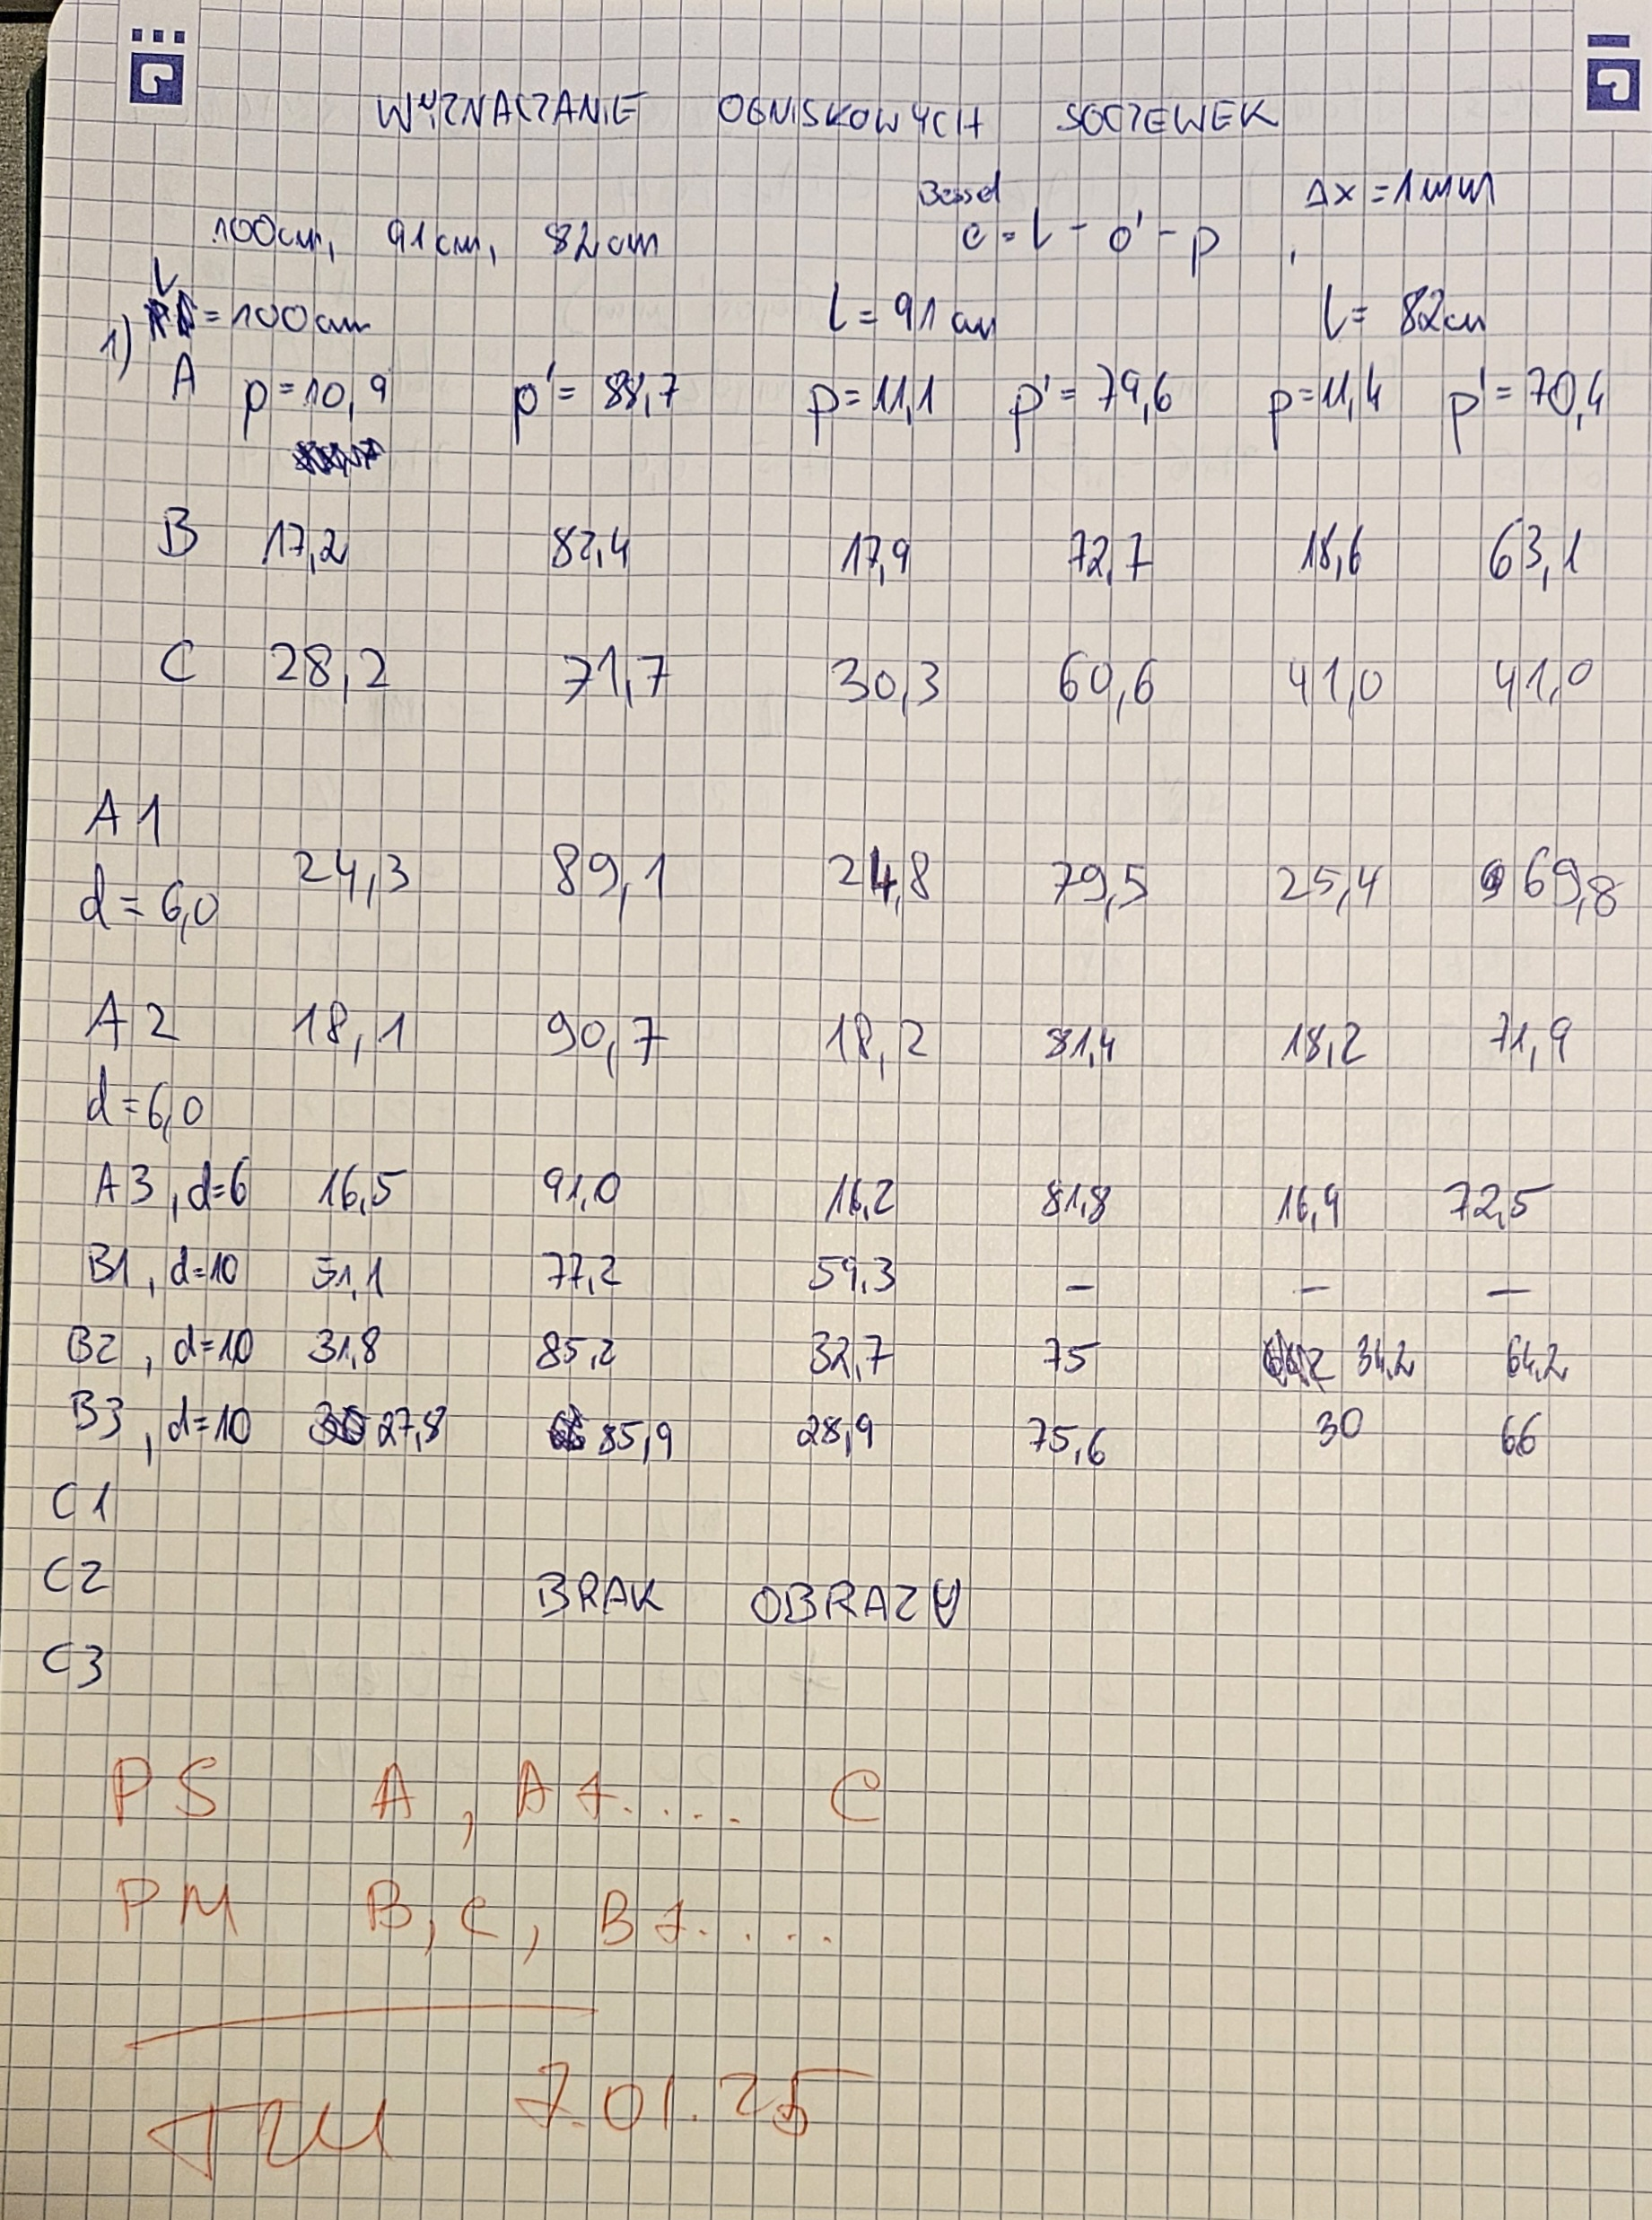
\includegraphics[scale=0.25]{images/pomiary.jpg}
\end{center}
% subsection Zdjecie wynikow pomiarow (end)

\section{Opracowanie wyników}\label{sec:opracowanie_wynikow} % (fold)

\subsection{Wzór soczewkowy}

\subsubsection{Obliczenia}\label{sec:obliczenia} % (fold)

Dla soczewki A i $l = 100cm$:
\[
	\frac{1}{f} = \frac{1}{p} + \frac{1}{o}
\]
\[
	f_A = \left( \frac{1}{10,9} + \frac{1}{89,1} \right)^{-1} = 9,7119 cm
\]
\paragraph{Soczewka A.}\label{par:soczewka_a} % (fold)
\mbox{} \\
\[
	\begin{array}{|c|c|c|c|c|c|c|c|c|}
		\hline
		l \, [cm]   & 100    & ~      & 91     & ~      & 82     & ~      \\ \hline
		p \, [cm]   & 10.9   & 88.7   & 11.1   & 79.6   & 11.4   & 70.4   \\ \hline
		o \, [cm]   & 89.1   & 11.3   & 79.9   & 11.4   & 70.6   & 11.6   \\ \hline
		f_A \, [cm] & 9.7119 & 10.023 & 9.7460 & 9.9718 & 9.8151 & 9.9590 \\ \hline
	\end{array}
\]
$$f_{AVG} = 9.871176 , \sigma = 0.119098 $$

% paragraph Soczewka A (end)

\paragraph{Soczewka C}\label{par:soczewka_c} % (fold)
\mbox{} \\
\[
	\begin{array}{|c|c|c|c|c|c|c|c|c|}
		\hline
		l \, [cm]   & 100     & ~       & 91     & ~      & 82   & ~    \\ \hline
		p \, [cm]   & 28.2    & 71.7    & 30.3   & 60.6   & 41   & 41   \\ \hline
		o \, [cm]   & 71.8    & 28.3    & 60.7   & 30.4   & 41   & 41   \\ \hline
		f_C \, [cm] & 20.2476 & 20.2911 & 20.211 & 20.244 & 20.5 & 20.5 \\ \hline
	\end{array}
\]
$$f_{AVG} = 20.332 , \sigma = 0.132 $$

% paragraph Soczewka C (end)

\paragraph{Układ A1}\label{par:paragraph_name} % (fold)
\mbox{} \\
\[
	\begin{array}{|c|c|c|c|c|c|c|c|c|}
		\hline
		l \, [cm]      & 100    & ~     & 91     & ~      & 82     & ~      \\ \hline
		p \, [cm]      & 24.3   & 89.1  & 24.8   & 79.5   & 25.4   & 69.8   \\ \hline
		o \, [cm]      & 75.7   & 10.9  & 66.2   & 11.5   & 56.6   & 12.2   \\ \hline
		f_{A1} \, [cm] & 18.395 & 9.711 & 18.041 & 10.046 & 17.532 & 10.384 \\ \hline
		f_{1} \, [cm]  & 8.154  & 7.057 & 8.127  & 7.125  & 8.085  & 7.190  \\ \hline
	\end{array}
\]
$$f_{AVG} = 7.6237047, \sigma = 0.548665 $$

% paragraph uklad A1 (end)

\paragraph{Układ A2}\label{par:paragraph_name} % (fold)
\mbox{} \\
\[
	\begin{array}{|c|c|c|c|c|c|c|c|c|}
		\hline
		l \, [cm]      & 100    & ~     & 91    & ~     & 82     & ~     \\ \hline
		p \, [cm]      & 18.1   & 90.7  & 18.2  & 81.4  & 18.2   & 71.9  \\ \hline
		o \, [cm]      & 81.9   & 9.3   & 72.8  & 9.599 & 63.8   & 10.1  \\ \hline
		f_{A2} \, [cm] & 14.823 & 8.435 & 14.56 & 8.587 & 14.160 & 8.855 \\ \hline
		f_2 \, [cm]    & 7.827  & 6.766 & 7.797 & 6.803 & 7.751  & 6.868 \\ \hline
	\end{array}
\]
$$f_{AVG} = 7.3026 , \sigma = 0.5380103 $$

% paragraph uklad A2 (end)

\paragraph{Układ A3}\label{par:paragraph_name} % (fold)
\mbox{} \\
\[
	\begin{array}{|c|c|c|c|c|c|c|c|c|}

		\hline
		l \, [cm] & 100    & ~     & 91     & ~     & 82     & ~     \\ \hline
		p \, [cm] & 16.5   & 91    & 16.2   & 81.8  & 16.9   & 72.5  \\ \hline
		o \, [cm] & 83.5   & 9     & 74.8   & 9.2   & 65.1   & 9.5   \\ \hline
		f \, [cm] & 13.777 & 8.19  & 13.316 & 8.269 & 13.416 & 8.399 \\ \hline
		f \, [cm] & 7.705  & 6.702 & 7.647  & 6.72  & 7.660  & 6.756 \\ \hline
	\end{array}
\]
$$f_{AVG} = 7.19970 , \sigma = 0.51751 $$

% paragraph uklad A3 (end)

% subsubsection Obliczenia (end)

\subsubsection{Wyniki}\label{sec:wyniki} % (fold)
\Large
\[
	f_A = 9,9 \pm 0,1 \, cm
\]
\[
	f_C = 20,33 \pm 0,13  \, cm
\]
\[
	f_1 = 7,6 \pm 0,5  \, cm
\]
\[
	f_2 = 7,3 \pm 0,5  \, cm
\]
\[
	f_2 = 7,2 \pm 0,5  \, cm
\]
\normalsize
% subsubsection Wyniki (end)

% subsection wzor soczewkowy (end)

\subsection{Metoda Bessela}

\subsubsection{Obliczenia}\label{sec:obliczenia} % (fold)

Dla soczewki A i $l = 100cm$:
\[
	e = l - o' - p
\]
\[
	f = \frac{l^2 - e^2}{4l}
\]
\[
	f_A = \frac{100^2 - (100 - 11,3 - 10,9)^2}{4 \cdot 100} = 9,867 m
\]

\paragraph{Soczewka A}\label{par:soczewka_a} % (fold)
\mbox{} \\
\[
	\begin{array}{|c|c|c|c|c|c|c|c|c|}
		\hline
		l \, [cm] & 100   & ~    & 91   & ~    & 82    & ~    \\ \hline
		p \, [cm] & 10.9  & 88.7 & 11.1 & 79.6 & 11.4  & 70.4 \\ \hline
		o \, [cm] & ~     & 11.3 & ~    & 11.4 & ~     & 11.6 \\ \hline
		e \, [cm] & 77.8  & ~    & 68.5 & ~    & 59    & ~    \\ \hline
		f \, [cm] & 9.867 & ~    & 9.85 & ~    & 9.887 & ~    \\ \hline
	\end{array}
\]
$$f_{AVG} = 9.8714 , \sigma = 0.01169 $$

% paragraph Soczewka A (end)

\paragraph{Soczewka C}\label{par:soczewka_c} % (fold)
\mbox{} \\
\[
	\begin{array}{|c|c|c|c|c|c|c|c|c|}
		\hline
		l \, [cm] & 100   & ~    & 91    & ~    & 82   & ~  \\ \hline
		p \, [cm] & 28.2  & 71.7 & 30.3  & 60.6 & 41   & 41 \\ \hline
		o \, [cm] & ~     & 28.3 & ~     & 30.4 & ~    & 41 \\ \hline
		e \, [cm] & 43.5  & ~    & 30.3  & ~    & 0    & ~  \\ \hline
		f \, [cm] & 20.26 & ~    & 20.22 & ~    & 20.5 & ~  \\ \hline
	\end{array}
\]
$$f_{AVG} = 20.33238 , \sigma = 0.11973 $$

% paragraph Soczewka C (end)

\paragraph{Układ A1}\label{par:paragraph_name} % (fold)
\mbox{} \\
\[
	\begin{array}{|c|c|c|c|c|c|c|c|c|}
		\hline
		l \, [cm]      & 100    & ~    & 91     & ~    & 82     & ~    \\ \hline
		p \, [cm]      & 24.3   & 89.1 & 24.8   & 79.5 & 25.4   & 69.8 \\ \hline
		o \, [cm]      & ~      & 10.9 & ~      & 11.5 & ~      & 12.2 \\ \hline
		e \, [cm]      & 64.8   & ~    & 54.7   & ~    & 44.4   & ~    \\ \hline
		f_{A1} \, [cm] & 14.502 & ~    & 14.529 & ~    & 14.489 & ~    \\ \hline
		f_1 \, [cm]    & 7.791  & ~    & 7.794  & ~    & 7.790  & ~    \\ \hline
	\end{array}
\]
$$f_{AVG} = 7.79204 , \sigma = 0.00189 $$

% paragraph uklad A1 (end)

\paragraph{Układ A2}\label{par:paragraph_name} % (fold)
\mbox{} \\
\[
	\begin{array}{|c|c|c|c|c|c|c|c|c|}
		\hline
		l \, [cm]      & 100    & ~    & 91     & ~    & 82     & ~    \\ \hline
		p \, [cm]      & 18.1   & 90.7 & 18.2   & 81.4 & 18.2   & 71.9 \\ \hline
		o \, [cm]      & ~      & 9.3  & ~      & 9.59 & ~      & 10.1 \\ \hline
		e \, [cm]      & 72.6   & ~    & 63.2   & ~    & 53.7   & ~    \\ \hline
		f_{A2} \, [cm] & 11.823 & ~    & 11.776 & ~    & 11.708 & ~    \\ \hline
		f_2 \, [cm]    & 7.436  & ~    & 7.429  & ~    & 7.418  & ~    \\ \hline
	\end{array}
\]
$$f_{AVG} =  7.428023 , \sigma = 0.00737 $$

% paragraph uklad A2 (end)

\paragraph{Układ A3}\label{par:paragraph_name} % (fold)
\mbox{} \\
\[
	\begin{array}{|c|c|c|c|c|c|c|c|c|}
		\hline
		l \, [cm]      & 100   & ~  & 91     & ~    & 82    & ~    \\ \hline
		p \, [cm]      & 16.5  & 91 & 16.2   & 81.8 & 16.9  & 72.5 \\ \hline
		o \, [cm]      & ~     & 9  & ~      & 9.2  & ~     & 9.5  \\ \hline
		e \, [cm]      & 74.5  & ~  & 65.6   & ~    & 55.6  & ~    \\ \hline
		f_{A3} \, [cm] & 11.12 & ~  & 10.927 & ~    & 11.07 & ~    \\ \hline
		f_3 \, [cm]    & 7.32  & ~  & 7.289  & ~    & 7.31  & ~    \\ \hline
	\end{array}
\]
$$f_{AVG} = 7.3088 , \sigma = 0.0144 $$

% paragraph uklad A3 (end)

% subsubsection Obliczenia (end)

\subsubsection{Wyniki}\label{sec:wyniki} % (fold)
\Large
\[
	f_A = 9,87 \pm 0,01 \, cm
\]
\[
	f_C = 20,3 \pm 0,1  \, cm
\]
\[
	f_1 = 7,792 \pm 0,002  \, cm
\]
\[
	f_2 = 7,428 \pm 0,007  \, cm
\]
\[
	f_2 = 7,309 \pm 0,014  \, cm
\]
\normalsize
% subsubsection Wyniki (end)


% subsection metoda bessela (end)

%section opracowanie wynikow

\section{Wnioski}\label{sec:wnioski} % (fold)
Wyznaczone wartości obarczone są dużymi niepewnościami, odychylenie standardowe średniej dla układu soczewek $A1$ wynosi ponad 4. Wynonie więszej ilośći pomiarów mogłoby poprawić dokładność. Metoda Bessela nie jest obarczona tak dużymi niepewnościami.
% section Wnioski (end)

\end{document}

